\documentclass[letterpaper,10pt]{book}
% Change to 10 pt
\usepackage{pdfpages}
\usepackage{morewrites}			% to counteract the no write space problem
\setcounter{tocdepth}{5}

\usepackage[framemethod=TikZ]{mdframed}

\usepackage{fancyhdr}

\usepackage{paralist}
\usepackage{amsmath}
\usepackage{amsfonts}
\usepackage{amssymb}
\usepackage{graphicx}

\usepackage{datetime}
%\usepackage{ulem}

%\usepackage[nottoc]{toobibind}

\usepackage[inline]{enumitem}

% Outer margin at 2.50 is exactly correct to fit the ``corruption alert'' tables
\usepackage[inner=1.0in, outer=2.50in, top=2.54cm,bottom=2.54cm, marginparwidth=2.25in]{geometry}

\usepackage{marginnote}
\usepackage{longtable}
\usepackage{booktabs}
\usepackage{xcolor}

\usepackage{soul}

\usepackage{marginnote}
\usepackage{imakeidx} 
\usepackage[
	backref=true,
	style=numeric,
%	citestyle=numeric,
	backend=bibtex
	]{biblatex}
\usepackage[driverfallback=hypertex,colorlinks=True]{hyperref}
\usepackage{cleveref}

\makeindex[name=scripture,columnsep=20pt, columnseprule=True,columns=3, title=Scripture References]
\makeindex[name=speaker,columnsep=20pt, columnseprule=True,,columns=2, title=Sermon Creator]
\makeindex[name=series,columnsep=20pt, columnseprule=True,,columns=2, title=Sermon Series]
\makeindex[name=date,columnsep=20pt, columnseprule=True,columns=2, title=Sermon Date]

\makeindex[name=event,columnsep=20pt, columnseprule=True,columns=2, title=Event]

\makeindex[name=topic,columnsep=20pt, columnseprule=True,columns=2, title=Topic]
\makeindex[name=AWIP,columnsep=20pt, columnseprule=True,columns=3, title=All Words in Passage]
\makeindex[name=NWIV,columnsep=20pt, columnseprule=True,columns=3, title=Number of Words in Verse]
\makeindex[name=PNIP,columnsep=20pt, columnseprule=True,columns=3, title=Proper Names in Passage]
\makeindex[name=PEIP,columnsep=20pt, columnseprule=True,columns=2, title=Prophetic Events in Passage]


\makeindex[name=TWPAQ,columnsep=20pt, columnseprule=True,columns=1, title=13-Word Phrases and Quotes]
\makeindex[name=PFTTIS,columnsep=20pt, columnseprule=False,columns=3, title=Phrases found 13 times in scripture]
\makeindex[name=WFTTIS,columnsep=20pt, columnseprule=False,columns=3, title=Words found 13 times in scripture]
\makeindex[name=WFITV,columnsep=20pt, columnseprule=False,columns=3, title=Words found in exactly 13 verses]
\makeindex[name=EVENTS,columnsep=20pt, columnseprule=False,columns=2, title=Sermon Log by Place]
\makeindex[name=QUESTIONS,columnsep=20pt, columnseprule=False,columns=2, title=Bible Questions]

\makeindex[name=DOCTRINES,columnsep=20pt, columnseprule=False,columns=2, title=Doctrines]

\makeindex[name=SONGS,columnsep=20pt, columnseprule=False,columns=1, title=Songs]
\makeindex[name=LOCATION,columnsep=20pt, columnseprule=False,columns= 2, title=Location]
\makeindex[name=FACEBOOK,columnsep=20pt, columnseprule=False,columns=2, title=Facebook]



\pagestyle{fancy}
\fancyhf{}
\fancyhead[LE,RO]{\today}
\fancyhead[RE,LO]{Notes, Outlines, Comments}
\fancyhead[CE,CO]{-page \thepage  - }

\fancyfoot[CO,CE]{\leftmark}
%\fancyfoot[LE,RO]{CSCE 692, HW1}

\title{DBR\\
Daily \\ Reads}
\author{Keith Anthony \\
\today }
%\title

%+/ffffff +   \pagenumbering{gobble}

\bibliography{Bibliographies/All20220108}

%%%%% TWEAKS:
%%% - distance from fcolorbox frame to text
\setlength{\fboxsep}{1.0pt}

\usepackage[utf8]{inputenc}
\usepackage{tikz}

%%%%%%%%%%%%%%%%%%%%%%%%%%%%%%%%%%%%%%%%%%%%%%%%%%%%%%%%%%%%%%%%%%%%%%%%%%%%%%%%

\begin{document}

\begin{titlepage}

% Set the text of the page to right-aligned until \end{flushright}
\begin{flushright}
\rightskip=-2.5cm

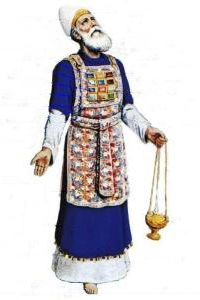
\includegraphics[width=50mm,scale=1.5]{Melchisedec.jpg}
\vspace{0.4in}

% Create a title for the document and write it in bold font
\LARGE{\textbf{\date}}
\linebreak

\vspace{0.5in}


\begin{flushleft}
\LARGE{Proverb 18\\}\vspace{0.25in}
\LARGE{Notes, Outlines, Comments}
\end{flushleft}

% write in large letters
%\large{Free webservices and apps}

% Skip some space
\vspace{0.6in}

%\large{Documentation}
% Skip some space

\bigskip

\normalsize{Xenia, Oh.\\}
\normalsize{created: \today}

% Skip some space
\vspace{1.3in}

\end{flushright}
% End the title page
\end{titlepage}

%\titlehttps://www.overleaf.com/project/60d732302fc633866943c9d2JE

\newpage 

\tableofcontents\hypertarget{TOC}{}
\listoffigures
\listoftables

\hyphenation{A-bim-e-lech bre-thren E-phra-im  Gib-e-o-nites Jer-u-sa-lem through-out Phil-i-stines The-o-phil-us Am-a-le-kites ven-geance Mesh-el-e-mi-ah onan-ism Phar-a-oh Py-thon thoughts grev-ous-ness Hach-a-liah adul-ter-er Shad-rach}

%\fcolorbox{black}{bone}{TEXT}
%%%%%%%%%%%%%%%%% EXTRA COLORS
%%%%%%%%%%%%%%%%% EXTRA COLORS
%%%%%%%%%%%%%%%%% EXTRA COLORS
\definecolor{champagne}{rgb}{0.97,0.91,0.81}
\definecolor{bone}{rgb}{0.89,0.85,0.79}

\definecolor{ForestGreen}{rgb}{0.00,0.29,0.098}
\definecolor{GIVING}{cmyk}{1,0.0,0.72,.1}

\definecolor{MLPE}{cmyk}{1,1,0,.45}
\definecolor{SOCCER}{cmyk}{.77, 0, .42, .49}
\definecolor{PAYBILL}{cmyk}{0,0.83,0.76,0.07}
\definecolor{SERMON}{cmyk}{.14,.9,0,.30} % aka seance \href{http://www.flatuicolorpicker.com/purple-cmyk-color-model/}{seance}
\definecolor{BIBLE}{cmyk}{0,.17,.74,.17}
\definecolor{WORKBLUE}{cmyk}{1, .5, 0, .6}
\definecolor{myOrange}{cmyk}{0, .4, .98, .03}
\definecolor{myTan}{cmyk}{0.0,.07,.17,.10}
\definecolor{myRed}{cmyk}{0,1,1,0}
\definecolor{myWhite}{cmyk}{0,0,0,0}
\definecolor{BLUESoD}{cmyk}{.97,.84,0,.04}
\definecolor{WHITE}{cmyk}{0,0,0,0}
\definecolor{OLDGOLD}{cmyk}{0.05,0.3,1.00,0}
\definecolor{CASTLETON}{cmyk}{1,0,0.31,0.66}
\definecolor{cadmiumgreen}{rgb}{0.0, 0.42, 0.24}
\definecolor{jungle}{rgb}{0.203,0.4882,0.1718}
\definecolor{MYGOLD}{rgb}{1,.84,0}

\definecolor{MYLIGHTGRAY}{rgb}{.85,.85,.85}

\definecolor{codegreen}{rgb}{0,0.6,0}
\definecolor{codegray}{rgb}{0.5,0.5,0.5}
\definecolor{codepurple}{rgb}{0.58,0,0.82}
\definecolor{backcolour}{rgb}{0.95,0.95,0.92}



\mdfdefinestyle{MyFrame}{%
    linecolor=blue,
    outerlinewidth=2pt,
    roundcorner=5pt,
    innertopmargin=\baselineskip,
    innerbottommargin=\baselineskip,
    innerrightmargin=10pt,
    innerleftmargin=10pt,
    backgroundcolor=gray!25!white}


\mdfdefinestyle{MyFrame2}{%
    linecolor=black,
    outerlinewidth=2pt,
    roundcorner=5pt,
    innertopmargin=\baselineskip,
    innerbottommargin=\baselineskip,
    innerrightmargin=10pt,
    innerleftmargin=10pt,
    backgroundcolor=yellow!25!white}



%\input{PFTTIS}
%\input{WFTTIS}
%\input{WFITV}



\chapter{Proverb 18}
\begin{figure}
  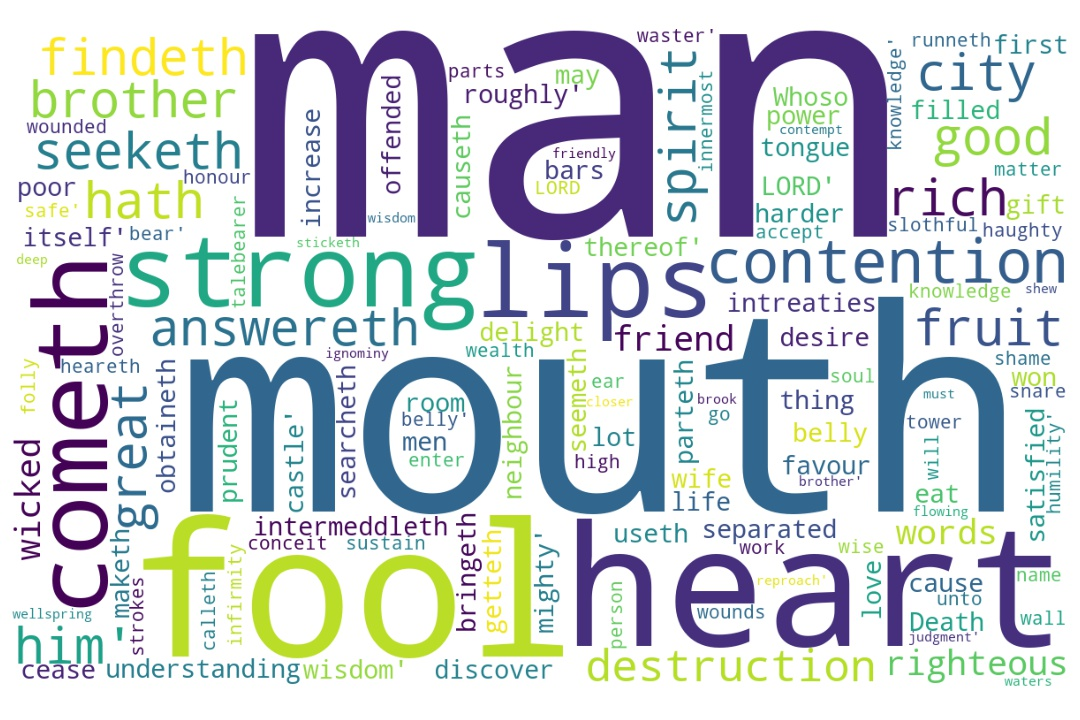
\includegraphics[width=\linewidth]{20OT-Proverbs/Proverb18-WordCloud.jpg}
  \caption{Proverb 18 Word Cloud}
  \label{fig:Proverb 18 word Cloud}
\end{figure}

\marginpar{\scriptsize \centering \fcolorbox{bone}{lime}{\textbf{A MAN FOCUSED ON GOD}}\\ (Proverbs 18:1-24) \begin{compactenum}[I.][8]
    \item Will be an \textbf{Inspired Man} - 
    \item Will be \textbf{Separate from the Ignorant Masses} - 
    \item For him most things in life will have  
    \textbf{Insignificant Meaning} - 
    \item Lives in an \textbf{Isolated Manner} 
    \item Lives by an \textbf{Individual Mandate} 
    \item Has an \textbf{intense and Insular Mentality}
\end{compactenum}}

\marginpar{\scriptsize \centering \fcolorbox{bone}{yellow}{\textbf{A FRIEND LIKE JESUS}}\\ (Proverb 18:24) \begin{compactenum}[I.][8]
    \item A \textbf{Close} Friend
    \item A \textbf{Constant} Friend
    \item A \textbf{Confiding} Friend
    \item A \textbf{Concerned} Friend
    \item A \textbf{Continuing} Friend
    \item A \textbf{Capable} Friend
    \item A \textbf{Caring} Friend
\end{compactenum}}

\marginpar{\scriptsize \centering \fcolorbox{bone}{black}{\textbf{\textcolor{white}{THE PURSUIT OF WISDOM}}}\\ (Proverb 18:24) \begin{compactenum}[I.][8]
    \item Then \textbf{Perverted} Motive -- to learn how manipulate events and circumstances. \index[scripture]{Proverbs!Pro 18:01}(Proverb 18:1)
    \item Then \textbf{Prideful} Motive -- To become exalted as wise. 
    \item Then \textbf{Public} Motive -- to be known and famous. 
    \item Then \textbf{Personal} Motive -- to achieve understanding. 
    \item Then \textbf{Practical} Motive -- to learn how live without mistakes or errors. 
    \item Then \textbf{Purposeful} Motive -- to learn navigate a specific problem. 
    \item Then \textbf{Perfect} Motive -- to learn how to live righteously before God. 
\end{compactenum}}

\marginpar{\scriptsize \centering \fcolorbox{bone}{blue}{\textbf{\textcolor{white}{WHAT YOUR SPEECH REVEALS}}}\\ (Proverb 18:4) \begin{compactenum}[I.][8]
    \item \textbf{Your Education} 
    \item \textbf{Your Excellence} 
    \item \textbf{Your Excitements} 
    \item \textbf{Your Enmity} 
    \item \textbf{Your Enemies} 
    \item \textbf{Your End} 
    \item \textbf{Your Emptiness}
    \item \textbf{Your Entanglements} 
\end{compactenum} }

\marginpar{\scriptsize \centering \fcolorbox{bone}{orange}{\textbf{THE WISE MAN}}\\ (Proverbs 18:1-24) \begin{compactenum}[I.][8]
    \item \textbf{Is Distinctive}
    \item \textbf{Is Disciplined}
    \item \textbf{Ignores Distractions}
    \item \textbf{Finds Delights in Wisdom}
    \item \textbf{Has Departed from the Common and Mundane}
    \item \textbf{Has a Distaste for Foolishness}
    \item \textbf{Is often regarded as Disturbed}
\end{compactenum} }




\footnote{\textcolor[cmyk]{0.99998,1,0,0}{\hyperlink{TOC}{Return to end of Table of Contents.}}}\footnote{\href{https://www.audioverse.org/english/audiobibles/books/ENGKJV/O/Prov/1}{\textcolor[cmyk]{0.99998,1,0,0}{Proverbs Audio}}}\textcolor[cmyk]{0.99998,1,0,0}{Through desire a man, having separated himself, seeketh \emph{and} \fcolorbox{bone}{MYGOLD}{intermeddleth} with all wisdom.}
[2] \textcolor[cmyk]{0.99998,1,0,0}{A fool hath no delight in \fcolorbox{bone}{MYGOLD}{understanding}, but that \fcolorbox{bone}{bone}{his} heart may discover itself.}
[3] \textcolor[cmyk]{0.99998,1,0,0}{When the wicked cometh, \emph{then} cometh also contempt, and with ignominy reproach.}
[4] \textcolor[cmyk]{0.99998,1,0,0}{The words of a man's mouth \emph{are} \emph{as} deep waters, \emph{and} the wellspring of wisdom \emph{as} a flowing brook.}\footnote{\textbf{Proverb 16:22} - Understanding is a wellspring of life unto him that hath it: but the instruction of fools is folly.}
[5] \textcolor[cmyk]{0.99998,1,0,0}{\emph{It} \emph{is} not good to accept the person of the wicked, to overthrow the righteous in judgment.}
[6] \textcolor[cmyk]{0.99998,1,0,0}{A fool's lips enter into contention, and \fcolorbox{bone}{bone}{his} mouth calleth for strokes.}
[7] \textcolor[cmyk]{0.99998,1,0,0}{A fool's mouth \emph{is} \fcolorbox{bone}{bone}{his} destruction, and \fcolorbox{bone}{bone}{his} lips \emph{are} the snare of \fcolorbox{bone}{bone}{his} soul.}
[8] \textcolor[cmyk]{0.99998,1,0,0}{The words of a talebearer \emph{are} as wounds, and they go down into the innermost parts of the belly.}
[9] \textcolor[cmyk]{0.99998,1,0,0}{He also that is slothful in \fcolorbox{bone}{bone}{his} work is brother to him that is a great waster.}
[10] \textcolor[cmyk]{0.99998,1,0,0}{The name of the LORD \emph{is} a strong tower: the righteous runneth into it, and is safe.}
[11] \textcolor[cmyk]{0.99998,1,0,0}{The rich man's wealth \emph{is} \fcolorbox{bone}{bone}{his} strong city, and as an high wall in \fcolorbox{bone}{bone}{his} own conceit.}
[12] \textcolor[cmyk]{0.99998,1,0,0}{Before destruction the heart of man is haughty, and before honour \emph{is} humility.}
[13] \textcolor[cmyk]{0.99998,1,0,0}{He that answereth a matter before he heareth \emph{it}, it \emph{is} folly and shame unto him.}
[14] \textcolor[cmyk]{0.99998,1,0,0}{The spirit of a man will sustain \fcolorbox{bone}{bone}{his} infirmity; but a wounded spirit who can bear?}
[15] \textcolor[cmyk]{0.99998,1,0,0}{The heart of the prudent getteth knowledge; and the ear of the wise seeketh knowledge.}
[16] \textcolor[cmyk]{0.99998,1,0,0}{A man's gift maketh room for him, and bringeth him before great men.}
[17] \textcolor[cmyk]{0.99998,1,0,0}{\emph{He} \emph{that} \emph{is} first in \fcolorbox{bone}{bone}{his} own cause \emph{seemeth} just; but \fcolorbox{bone}{bone}{his} neighbour cometh and searcheth him.}
[18] \textcolor[cmyk]{0.99998,1,0,0}{The lot causeth contentions to cease, and parteth between the mighty.}
[19] \textcolor[cmyk]{0.99998,1,0,0}{A brother offended \emph{is} \emph{harder} \emph{to} \emph{be} \emph{won} than a strong city: and \emph{their} contentions \emph{are} like the bars of a castle.}
[20] \textcolor[cmyk]{0.99998,1,0,0}{A man's belly shall be satisfied with the fruit of \fcolorbox{bone}{bone}{his} mouth; \emph{and} with the increase of \fcolorbox{bone}{bone}{his} lips shall he be filled.}
[21] \textcolor[cmyk]{0.99998,1,0,0}{Death and life \emph{are} in the power of the tongue: and they that love it shall eat the fruit thereof.}
[22] \textcolor[cmyk]{0.99998,1,0,0}{\emph{Whoso} findeth a wife findeth a good \emph{thing}, and obtaineth favour of the LORD.}
[23] \textcolor[cmyk]{0.99998,1,0,0}{The poor useth intreaties; but the rich answereth roughly.}
[24] \textcolor[cmyk]{0.99998,1,0,0}{A man \emph{that} \emph{hath} friends must shew himself friendly: and there is a friend \emph{that} sticketh closer than a brother.}



\section{Proverb 18 Comments}

\subsection{Numerical Nuggets}
\textbf{13:} The word ``wellspring'' found only twice in scripture is the 13$^{th}$ word in verse 4. Two thirteen-letter words are in the chapter: ``intermeddleth'' and ``understanding.'' Verse 12, speaking of haughtiness, has 13 words. Verses 1, 12, and 16 have 13 words. Verses 7 and 12 have 13 unique words. The word ``his'' is used 13 times in the chapter. The 13-letter words ``intermeddleth'' and ``understanding'' are used in the chapter.

\subsection{Proverb 18:1-2}
The issue addressed in verses 1 and 2 is the human heart, and as such it should be expected that man will confront and change it, as shown in Table~\ref{table:CorruptionProv18:1}. The verse goes to motive. This is why most (or maybe all) research, ostensibly done for the betterment of mankind, eventually is used to oppress mankind. It comes down to power, position, prestige, prominence, and power. It comes down to why one seeks those things. Verse 2 puts the thought in context: it is the fool who trusts his heart and seeks the heart's desire. Why is this man a fool? It is because a sincere, God-seeking man will quickly elan from scripture the sordid details and depravity of the human heart.\footnote{\textbf{Isaiah 5:21} - Woe unto them that are wise in their own eyes, and prudent in their own sight!}\footnote{\textbf{Luke 10:21} - In that hour Jesus rejoiced in spirit, and said, I thank thee, O Father, Lord of heaven and earth, that thou hast hid these things from the wise and prudent, and hast revealed them unto babes: even so, Father; for so it seemed good in thy sight.}\\
\\
\noindent One commentator explains the process \cite{ruckman1972proverbs}:
\begin{compactenum}[1.]
    \item DESIRE is at the root of all scientific research and investigation (verse 1),
    \item This desire comes form the human HEART and not the human MIND (verse 2),
    \item This desire is essentially subjective, egotistical, and self-seeking (verse 2),
    \item This desire leads a man to pursue the life of isolated superiority, perhaps even the ivory towers of academic, or the esteemed halls of theological institutions, where he deep-down considers himself to be above the masses, or above the common folk. This may even start out as, or continue to masquerade as, a noble cause.
    \item The man does not seek wisdom. He ``seeketh and intermeddleth with all wisdom.'' 
    \item The man's ``love of wisdom'' is neither pure, not objective, not philanthropic.
    \item The wisdom ``sought'' is complete and is a mean's to an end.
\end{compactenum}

\newpage
\begin{center}

\begin{table}[ht]
\centering
\begin{tabular}{|p{.5in}|p{3.5in}|}
    \hline
    \textcolor{blue}{AV} & \textcolor{blue}{Through desire a man, having separated himself, seeketh \emph{and} intermeddleth with all wisdom.}\\ \hline
    \hline
    CEB &  Unfriendly people look out for themselves; they bicker with sensible people.\\ \hline
%
ESV & Whoever isolates himself seeks his own desire;  he breaks out against all sound judgment. \\ \hline
%
NASV &  He who separates himself seeks his own desire, He quarrels against all sound wisdom.\\ \hline
%
MEV & He who separates himself seeks his own desire; he seeks and quarrels against all wisdom.\\ \hline
%
NIV &  An unfriendly person pursues selfish ends and against all sound judgment starts quarrels. \\ \hline
%
NKJV &  A man who isolates himself seeks his own desire; He rages against all wise judgment.\\ \hline
%
RSV &  He who is estranged seeks pretexts  to break out against all sound judgment.\\ \hline \hline

\multicolumn{2}{|p{4.2in}|}{{\textcolor{jungle}{Modern translations, such as the ASV and others, strike out the first part of the verse, concealing the intent of mankind in general.  It goes to the heart's intent in seeking wisdom. How wonderful is the obfuscated RSV text: ``He who is estranged seeks pretexts.'' What does THAT mean?}}} \\ \hline

\end{tabular}
\caption[Corruption Alert: Proverb 18:1]{Corruption Alert: Proverb 18:1} \label{table:Corruption Proverb 18:1}
\end{table}

\end{center}


\newpage


%\index[NWIV]{13!Proverbs!Pro 18:1}\index[AWIP]{Through!Proverbs!Pro 18:1}\index[AWIP]{desire!Proverbs!Pro 18:1}\index[AWIP]{a!Proverbs!Pro 18:1}\index[AWIP]{man!Proverbs!Pro 18:1}\index[AWIP]{having!Proverbs!Pro 18:1}\index[AWIP]{separated!Proverbs!Pro 18:1}\index[AWIP]{himself!Proverbs!Pro 18:1}\index[AWIP]{seeketh!Proverbs!Pro 18:1}\index[AWIP]{\emph{and}!Proverbs!Pro 18:1}\index[AWIP]{intermeddleth!Proverbs!Pro 18:1}\index[AWIP]{with!Proverbs!Pro 18:1}\index[AWIP]{all!Proverbs!Pro 18:1}\index[AWIP]{wisdom!Proverbs!Pro 18:1}\index[AWIP]{\emph{and}!Proverbs!Pro 18:1}

\index[NWIV]{14!Proverbs!Pro 18:2}\index[AWIP]{A!Proverbs!Pro 18:2}\index[AWIP]{fool!Proverbs!Pro 18:2}\index[AWIP]{hath!Proverbs!Pro 18:2}\index[AWIP]{no!Proverbs!Pro 18:2}\index[AWIP]{delight!Proverbs!Pro 18:2}\index[AWIP]{in!Proverbs!Pro 18:2}\index[AWIP]{understanding!Proverbs!Pro 18:2}\index[AWIP]{but!Proverbs!Pro 18:2}\index[AWIP]{that!Proverbs!Pro 18:2}\index[AWIP]{his!Proverbs!Pro 18:2}\index[AWIP]{heart!Proverbs!Pro 18:2}\index[AWIP]{may!Proverbs!Pro 18:2}\index[AWIP]{discover!Proverbs!Pro 18:2}\index[AWIP]{itself!Proverbs!Pro 18:2}

\index[NWIV]{12!Proverbs!Pro 18:3}\index[AWIP]{When!Proverbs!Pro 18:3}\index[AWIP]{the!Proverbs!Pro 18:3}\index[AWIP]{wicked!Proverbs!Pro 18:3}\index[AWIP]{cometh!Proverbs!Pro 18:3}\index[AWIP]{cometh!Proverbs!Pro 18:3 (2)}\index[AWIP]{\emph{then}!Proverbs!Pro 18:3}\index[AWIP]{also!Proverbs!Pro 18:3}\index[AWIP]{contempt!Proverbs!Pro 18:3}\index[AWIP]{and!Proverbs!Pro 18:3}\index[AWIP]{with!Proverbs!Pro 18:3}\index[AWIP]{ignominy!Proverbs!Pro 18:3}\index[AWIP]{reproach!Proverbs!Pro 18:3}\index[AWIP]{\emph{then}!Proverbs!Pro 18:3}

\index[NWIV]{19!Proverbs!Pro 18:4}\index[AWIP]{The!Proverbs!Pro 18:4}\index[AWIP]{words!Proverbs!Pro 18:4}\index[AWIP]{of!Proverbs!Pro 18:4}\index[AWIP]{of!Proverbs!Pro 18:4 (2)}\index[AWIP]{a!Proverbs!Pro 18:4}\index[AWIP]{a!Proverbs!Pro 18:4 (2)}\index[AWIP]{man's!Proverbs!Pro 18:4}\index[AWIP]{mouth!Proverbs!Pro 18:4}\index[AWIP]{\emph{are}!Proverbs!Pro 18:4}\index[AWIP]{\emph{as}!Proverbs!Pro 18:4}\index[AWIP]{\emph{as}!Proverbs!Pro 18:4 (2)}\index[AWIP]{deep!Proverbs!Pro 18:4}\index[AWIP]{waters!Proverbs!Pro 18:4}\index[AWIP]{\emph{and}!Proverbs!Pro 18:4}\index[AWIP]{the!Proverbs!Pro 18:4}\index[AWIP]{wellspring!Proverbs!Pro 18:4}\index[AWIP]{wisdom!Proverbs!Pro 18:4}\index[AWIP]{flowing!Proverbs!Pro 18:4}\index[AWIP]{brook!Proverbs!Pro 18:4}\index[AWIP]{\emph{are}!Proverbs!Pro 18:4}\index[AWIP]{\emph{as}!Proverbs!Pro 18:4}\index[AWIP]{\emph{as}!Proverbs!Pro 18:4 (2)}\index[AWIP]{\emph{and}!Proverbs!Pro 18:4}

\index[NWIV]{17!Proverbs!Pro 18:5}\index[AWIP]{\emph{It}!Proverbs!Pro 18:5}\index[AWIP]{\emph{is}!Proverbs!Pro 18:5}\index[AWIP]{not!Proverbs!Pro 18:5}\index[AWIP]{good!Proverbs!Pro 18:5}\index[AWIP]{to!Proverbs!Pro 18:5}\index[AWIP]{to!Proverbs!Pro 18:5 (2)}\index[AWIP]{accept!Proverbs!Pro 18:5}\index[AWIP]{the!Proverbs!Pro 18:5}\index[AWIP]{the!Proverbs!Pro 18:5 (2)}\index[AWIP]{the!Proverbs!Pro 18:5 (3)}\index[AWIP]{person!Proverbs!Pro 18:5}\index[AWIP]{of!Proverbs!Pro 18:5}\index[AWIP]{wicked!Proverbs!Pro 18:5}\index[AWIP]{overthrow!Proverbs!Pro 18:5}\index[AWIP]{righteous!Proverbs!Pro 18:5}\index[AWIP]{in!Proverbs!Pro 18:5}\index[AWIP]{judgment!Proverbs!Pro 18:5}\index[AWIP]{\emph{It}!Proverbs!Pro 18:5}\index[AWIP]{\emph{is}!Proverbs!Pro 18:5}

\index[NWIV]{12!Proverbs!Pro 18:6}\index[AWIP]{A!Proverbs!Pro 18:6}\index[AWIP]{fool's!Proverbs!Pro 18:6}\index[AWIP]{lips!Proverbs!Pro 18:6}\index[AWIP]{enter!Proverbs!Pro 18:6}\index[AWIP]{into!Proverbs!Pro 18:6}\index[AWIP]{contention!Proverbs!Pro 18:6}\index[AWIP]{and!Proverbs!Pro 18:6}\index[AWIP]{his!Proverbs!Pro 18:6}\index[AWIP]{mouth!Proverbs!Pro 18:6}\index[AWIP]{calleth!Proverbs!Pro 18:6}\index[AWIP]{for!Proverbs!Pro 18:6}\index[AWIP]{strokes!Proverbs!Pro 18:6}

\index[NWIV]{15!Proverbs!Pro 18:7}\index[AWIP]{A!Proverbs!Pro 18:7}\index[AWIP]{fool's!Proverbs!Pro 18:7}\index[AWIP]{mouth!Proverbs!Pro 18:7}\index[AWIP]{\emph{is}!Proverbs!Pro 18:7}\index[AWIP]{his!Proverbs!Pro 18:7}\index[AWIP]{his!Proverbs!Pro 18:7 (2)}\index[AWIP]{his!Proverbs!Pro 18:7 (3)}\index[AWIP]{destruction!Proverbs!Pro 18:7}\index[AWIP]{and!Proverbs!Pro 18:7}\index[AWIP]{lips!Proverbs!Pro 18:7}\index[AWIP]{\emph{are}!Proverbs!Pro 18:7}\index[AWIP]{the!Proverbs!Pro 18:7}\index[AWIP]{snare!Proverbs!Pro 18:7}\index[AWIP]{of!Proverbs!Pro 18:7}\index[AWIP]{soul!Proverbs!Pro 18:7}\index[AWIP]{\emph{is}!Proverbs!Pro 18:7}\index[AWIP]{\emph{are}!Proverbs!Pro 18:7}

\index[NWIV]{19!Proverbs!Pro 18:8}\index[AWIP]{The!Proverbs!Pro 18:8}\index[AWIP]{words!Proverbs!Pro 18:8}\index[AWIP]{of!Proverbs!Pro 18:8}\index[AWIP]{of!Proverbs!Pro 18:8 (2)}\index[AWIP]{a!Proverbs!Pro 18:8}\index[AWIP]{talebearer!Proverbs!Pro 18:8}\index[AWIP]{\emph{are}!Proverbs!Pro 18:8}\index[AWIP]{as!Proverbs!Pro 18:8}\index[AWIP]{wounds!Proverbs!Pro 18:8}\index[AWIP]{and!Proverbs!Pro 18:8}\index[AWIP]{they!Proverbs!Pro 18:8}\index[AWIP]{go!Proverbs!Pro 18:8}\index[AWIP]{down!Proverbs!Pro 18:8}\index[AWIP]{into!Proverbs!Pro 18:8}\index[AWIP]{the!Proverbs!Pro 18:8}\index[AWIP]{the!Proverbs!Pro 18:8 (2)}\index[AWIP]{innermost!Proverbs!Pro 18:8}\index[AWIP]{parts!Proverbs!Pro 18:8}\index[AWIP]{belly!Proverbs!Pro 18:8}\index[AWIP]{\emph{are}!Proverbs!Pro 18:8}

\index[NWIV]{17!Proverbs!Pro 18:9}\index[AWIP]{He!Proverbs!Pro 18:9}\index[AWIP]{also!Proverbs!Pro 18:9}\index[AWIP]{that!Proverbs!Pro 18:9}\index[AWIP]{that!Proverbs!Pro 18:9 (2)}\index[AWIP]{is!Proverbs!Pro 18:9}\index[AWIP]{is!Proverbs!Pro 18:9 (2)}\index[AWIP]{is!Proverbs!Pro 18:9 (3)}\index[AWIP]{slothful!Proverbs!Pro 18:9}\index[AWIP]{in!Proverbs!Pro 18:9}\index[AWIP]{his!Proverbs!Pro 18:9}\index[AWIP]{work!Proverbs!Pro 18:9}\index[AWIP]{brother!Proverbs!Pro 18:9}\index[AWIP]{to!Proverbs!Pro 18:9}\index[AWIP]{him!Proverbs!Pro 18:9}\index[AWIP]{a!Proverbs!Pro 18:9}\index[AWIP]{great!Proverbs!Pro 18:9}\index[AWIP]{waster!Proverbs!Pro 18:9}

\index[NWIV]{17!Proverbs!Pro 18:10}\index[AWIP]{The!Proverbs!Pro 18:10}\index[AWIP]{name!Proverbs!Pro 18:10}\index[AWIP]{of!Proverbs!Pro 18:10}\index[AWIP]{the!Proverbs!Pro 18:10}\index[AWIP]{the!Proverbs!Pro 18:10 (2)}\index[AWIP]{LORD!Proverbs!Pro 18:10}\index[AWIP]{\emph{is}!Proverbs!Pro 18:10}\index[AWIP]{a!Proverbs!Pro 18:10}\index[AWIP]{strong!Proverbs!Pro 18:10}\index[AWIP]{tower!Proverbs!Pro 18:10}\index[AWIP]{righteous!Proverbs!Pro 18:10}\index[AWIP]{runneth!Proverbs!Pro 18:10}\index[AWIP]{into!Proverbs!Pro 18:10}\index[AWIP]{it!Proverbs!Pro 18:10}\index[AWIP]{and!Proverbs!Pro 18:10}\index[AWIP]{is!Proverbs!Pro 18:10}\index[AWIP]{safe!Proverbs!Pro 18:10}\index[AWIP]{\emph{is}!Proverbs!Pro 18:10}

\index[NWIV]{17!Proverbs!Pro 18:11}\index[AWIP]{The!Proverbs!Pro 18:11}\index[AWIP]{rich!Proverbs!Pro 18:11}\index[AWIP]{man's!Proverbs!Pro 18:11}\index[AWIP]{wealth!Proverbs!Pro 18:11}\index[AWIP]{\emph{is}!Proverbs!Pro 18:11}\index[AWIP]{his!Proverbs!Pro 18:11}\index[AWIP]{his!Proverbs!Pro 18:11 (2)}\index[AWIP]{strong!Proverbs!Pro 18:11}\index[AWIP]{city!Proverbs!Pro 18:11}\index[AWIP]{and!Proverbs!Pro 18:11}\index[AWIP]{as!Proverbs!Pro 18:11}\index[AWIP]{an!Proverbs!Pro 18:11}\index[AWIP]{high!Proverbs!Pro 18:11}\index[AWIP]{wall!Proverbs!Pro 18:11}\index[AWIP]{in!Proverbs!Pro 18:11}\index[AWIP]{own!Proverbs!Pro 18:11}\index[AWIP]{conceit!Proverbs!Pro 18:11}\index[AWIP]{\emph{is}!Proverbs!Pro 18:11}

\index[NWIV]{13!Proverbs!Pro 18:12}\index[AWIP]{Before!Proverbs!Pro 18:12}\index[AWIP]{destruction!Proverbs!Pro 18:12}\index[AWIP]{the!Proverbs!Pro 18:12}\index[AWIP]{heart!Proverbs!Pro 18:12}\index[AWIP]{of!Proverbs!Pro 18:12}\index[AWIP]{man!Proverbs!Pro 18:12}\index[AWIP]{is!Proverbs!Pro 18:12}\index[AWIP]{haughty!Proverbs!Pro 18:12}\index[AWIP]{and!Proverbs!Pro 18:12}\index[AWIP]{before!Proverbs!Pro 18:12}\index[AWIP]{honour!Proverbs!Pro 18:12}\index[AWIP]{\emph{is}!Proverbs!Pro 18:12}\index[AWIP]{humility!Proverbs!Pro 18:12}\index[AWIP]{\emph{is}!Proverbs!Pro 18:12}

\index[NWIV]{16!Proverbs!Pro 18:13}\index[AWIP]{He!Proverbs!Pro 18:13}\index[AWIP]{that!Proverbs!Pro 18:13}\index[AWIP]{answereth!Proverbs!Pro 18:13}\index[AWIP]{a!Proverbs!Pro 18:13}\index[AWIP]{matter!Proverbs!Pro 18:13}\index[AWIP]{before!Proverbs!Pro 18:13}\index[AWIP]{he!Proverbs!Pro 18:13}\index[AWIP]{heareth!Proverbs!Pro 18:13}\index[AWIP]{\emph{it}!Proverbs!Pro 18:13}\index[AWIP]{it!Proverbs!Pro 18:13}\index[AWIP]{\emph{is}!Proverbs!Pro 18:13}\index[AWIP]{folly!Proverbs!Pro 18:13}\index[AWIP]{and!Proverbs!Pro 18:13}\index[AWIP]{shame!Proverbs!Pro 18:13}\index[AWIP]{unto!Proverbs!Pro 18:13}\index[AWIP]{him!Proverbs!Pro 18:13}\index[AWIP]{\emph{it}!Proverbs!Pro 18:13}\index[AWIP]{\emph{is}!Proverbs!Pro 18:13}

\index[NWIV]{16!Proverbs!Pro 18:14}\index[AWIP]{The!Proverbs!Pro 18:14}\index[AWIP]{spirit!Proverbs!Pro 18:14}\index[AWIP]{spirit!Proverbs!Pro 18:14 (2)}\index[AWIP]{of!Proverbs!Pro 18:14}\index[AWIP]{a!Proverbs!Pro 18:14}\index[AWIP]{a!Proverbs!Pro 18:14 (2)}\index[AWIP]{man!Proverbs!Pro 18:14}\index[AWIP]{will!Proverbs!Pro 18:14}\index[AWIP]{sustain!Proverbs!Pro 18:14}\index[AWIP]{his!Proverbs!Pro 18:14}\index[AWIP]{infirmity!Proverbs!Pro 18:14}\index[AWIP]{but!Proverbs!Pro 18:14}\index[AWIP]{wounded!Proverbs!Pro 18:14}\index[AWIP]{who!Proverbs!Pro 18:14}\index[AWIP]{can!Proverbs!Pro 18:14}\index[AWIP]{bear?!Proverbs!Pro 18:14}

\index[NWIV]{15!Proverbs!Pro 18:15}\index[AWIP]{The!Proverbs!Pro 18:15}\index[AWIP]{heart!Proverbs!Pro 18:15}\index[AWIP]{of!Proverbs!Pro 18:15}\index[AWIP]{of!Proverbs!Pro 18:15 (2)}\index[AWIP]{the!Proverbs!Pro 18:15}\index[AWIP]{the!Proverbs!Pro 18:15 (2)}\index[AWIP]{the!Proverbs!Pro 18:15 (3)}\index[AWIP]{prudent!Proverbs!Pro 18:15}\index[AWIP]{getteth!Proverbs!Pro 18:15}\index[AWIP]{knowledge!Proverbs!Pro 18:15}\index[AWIP]{knowledge!Proverbs!Pro 18:15 (2)}\index[AWIP]{and!Proverbs!Pro 18:15}\index[AWIP]{ear!Proverbs!Pro 18:15}\index[AWIP]{wise!Proverbs!Pro 18:15}\index[AWIP]{seeketh!Proverbs!Pro 18:15}

\index[NWIV]{13!Proverbs!Pro 18:16}\index[AWIP]{A!Proverbs!Pro 18:16}\index[AWIP]{man's!Proverbs!Pro 18:16}\index[AWIP]{gift!Proverbs!Pro 18:16}\index[AWIP]{maketh!Proverbs!Pro 18:16}\index[AWIP]{room!Proverbs!Pro 18:16}\index[AWIP]{for!Proverbs!Pro 18:16}\index[AWIP]{him!Proverbs!Pro 18:16}\index[AWIP]{him!Proverbs!Pro 18:16 (2)}\index[AWIP]{and!Proverbs!Pro 18:16}\index[AWIP]{bringeth!Proverbs!Pro 18:16}\index[AWIP]{before!Proverbs!Pro 18:16}\index[AWIP]{great!Proverbs!Pro 18:16}\index[AWIP]{men!Proverbs!Pro 18:16}

\index[NWIV]{17!Proverbs!Pro 18:17}\index[AWIP]{\emph{He}!Proverbs!Pro 18:17}\index[AWIP]{\emph{that}!Proverbs!Pro 18:17}\index[AWIP]{\emph{is}!Proverbs!Pro 18:17}\index[AWIP]{first!Proverbs!Pro 18:17}\index[AWIP]{in!Proverbs!Pro 18:17}\index[AWIP]{his!Proverbs!Pro 18:17}\index[AWIP]{his!Proverbs!Pro 18:17 (2)}\index[AWIP]{own!Proverbs!Pro 18:17}\index[AWIP]{cause!Proverbs!Pro 18:17}\index[AWIP]{\emph{seemeth}!Proverbs!Pro 18:17}\index[AWIP]{just!Proverbs!Pro 18:17}\index[AWIP]{but!Proverbs!Pro 18:17}\index[AWIP]{neighbour!Proverbs!Pro 18:17}\index[AWIP]{cometh!Proverbs!Pro 18:17}\index[AWIP]{and!Proverbs!Pro 18:17}\index[AWIP]{searcheth!Proverbs!Pro 18:17}\index[AWIP]{him!Proverbs!Pro 18:17}\index[AWIP]{\emph{He}!Proverbs!Pro 18:17}\index[AWIP]{\emph{that}!Proverbs!Pro 18:17}\index[AWIP]{\emph{is}!Proverbs!Pro 18:17}\index[AWIP]{\emph{seemeth}!Proverbs!Pro 18:17}

\index[NWIV]{11!Proverbs!Pro 18:18}\index[AWIP]{The!Proverbs!Pro 18:18}\index[AWIP]{lot!Proverbs!Pro 18:18}\index[AWIP]{causeth!Proverbs!Pro 18:18}\index[AWIP]{contentions!Proverbs!Pro 18:18}\index[AWIP]{to!Proverbs!Pro 18:18}\index[AWIP]{cease!Proverbs!Pro 18:18}\index[AWIP]{and!Proverbs!Pro 18:18}\index[AWIP]{parteth!Proverbs!Pro 18:18}\index[AWIP]{between!Proverbs!Pro 18:18}\index[AWIP]{the!Proverbs!Pro 18:18}\index[AWIP]{mighty!Proverbs!Pro 18:18}

\index[NWIV]{22!Proverbs!Pro 18:19}\index[AWIP]{A!Proverbs!Pro 18:19}\index[AWIP]{brother!Proverbs!Pro 18:19}\index[AWIP]{offended!Proverbs!Pro 18:19}\index[AWIP]{\emph{is}!Proverbs!Pro 18:19}\index[AWIP]{\emph{harder}!Proverbs!Pro 18:19}\index[AWIP]{\emph{to}!Proverbs!Pro 18:19}\index[AWIP]{\emph{be}!Proverbs!Pro 18:19}\index[AWIP]{\emph{won}!Proverbs!Pro 18:19}\index[AWIP]{than!Proverbs!Pro 18:19}\index[AWIP]{a!Proverbs!Pro 18:19}\index[AWIP]{a!Proverbs!Pro 18:19 (2)}\index[AWIP]{strong!Proverbs!Pro 18:19}\index[AWIP]{city!Proverbs!Pro 18:19}\index[AWIP]{and!Proverbs!Pro 18:19}\index[AWIP]{\emph{their}!Proverbs!Pro 18:19}\index[AWIP]{contentions!Proverbs!Pro 18:19}\index[AWIP]{\emph{are}!Proverbs!Pro 18:19}\index[AWIP]{like!Proverbs!Pro 18:19}\index[AWIP]{the!Proverbs!Pro 18:19}\index[AWIP]{bars!Proverbs!Pro 18:19}\index[AWIP]{of!Proverbs!Pro 18:19}\index[AWIP]{castle!Proverbs!Pro 18:19}\index[AWIP]{\emph{is}!Proverbs!Pro 18:19}\index[AWIP]{\emph{harder}!Proverbs!Pro 18:19}\index[AWIP]{\emph{to}!Proverbs!Pro 18:19}\index[AWIP]{\emph{be}!Proverbs!Pro 18:19}\index[AWIP]{\emph{won}!Proverbs!Pro 18:19}\index[AWIP]{\emph{their}!Proverbs!Pro 18:19}\index[AWIP]{\emph{are}!Proverbs!Pro 18:19}

\index[NWIV]{23!Proverbs!Pro 18:20}\index[AWIP]{A!Proverbs!Pro 18:20}\index[AWIP]{man's!Proverbs!Pro 18:20}\index[AWIP]{belly!Proverbs!Pro 18:20}\index[AWIP]{shall!Proverbs!Pro 18:20}\index[AWIP]{shall!Proverbs!Pro 18:20 (2)}\index[AWIP]{be!Proverbs!Pro 18:20}\index[AWIP]{be!Proverbs!Pro 18:20 (2)}\index[AWIP]{satisfied!Proverbs!Pro 18:20}\index[AWIP]{with!Proverbs!Pro 18:20}\index[AWIP]{with!Proverbs!Pro 18:20 (2)}\index[AWIP]{the!Proverbs!Pro 18:20}\index[AWIP]{the!Proverbs!Pro 18:20 (2)}\index[AWIP]{fruit!Proverbs!Pro 18:20}\index[AWIP]{of!Proverbs!Pro 18:20}\index[AWIP]{of!Proverbs!Pro 18:20 (2)}\index[AWIP]{his!Proverbs!Pro 18:20}\index[AWIP]{his!Proverbs!Pro 18:20 (2)}\index[AWIP]{mouth!Proverbs!Pro 18:20}\index[AWIP]{\emph{and}!Proverbs!Pro 18:20}\index[AWIP]{increase!Proverbs!Pro 18:20}\index[AWIP]{lips!Proverbs!Pro 18:20}\index[AWIP]{he!Proverbs!Pro 18:20}\index[AWIP]{filled!Proverbs!Pro 18:20}\index[AWIP]{\emph{and}!Proverbs!Pro 18:20}

\index[NWIV]{20!Proverbs!Pro 18:21}\index[AWIP]{Death!Proverbs!Pro 18:21}\index[AWIP]{and!Proverbs!Pro 18:21}\index[AWIP]{and!Proverbs!Pro 18:21 (2)}\index[AWIP]{life!Proverbs!Pro 18:21}\index[AWIP]{\emph{are}!Proverbs!Pro 18:21}\index[AWIP]{in!Proverbs!Pro 18:21}\index[AWIP]{the!Proverbs!Pro 18:21}\index[AWIP]{the!Proverbs!Pro 18:21 (2)}\index[AWIP]{the!Proverbs!Pro 18:21 (3)}\index[AWIP]{power!Proverbs!Pro 18:21}\index[AWIP]{of!Proverbs!Pro 18:21}\index[AWIP]{tongue!Proverbs!Pro 18:21}\index[AWIP]{they!Proverbs!Pro 18:21}\index[AWIP]{that!Proverbs!Pro 18:21}\index[AWIP]{love!Proverbs!Pro 18:21}\index[AWIP]{it!Proverbs!Pro 18:21}\index[AWIP]{shall!Proverbs!Pro 18:21}\index[AWIP]{eat!Proverbs!Pro 18:21}\index[AWIP]{fruit!Proverbs!Pro 18:21}\index[AWIP]{thereof!Proverbs!Pro 18:21}\index[AWIP]{\emph{are}!Proverbs!Pro 18:21}

\index[NWIV]{14!Proverbs!Pro 18:22}\index[AWIP]{\emph{Whoso}!Proverbs!Pro 18:22}\index[AWIP]{findeth!Proverbs!Pro 18:22}\index[AWIP]{findeth!Proverbs!Pro 18:22 (2)}\index[AWIP]{a!Proverbs!Pro 18:22}\index[AWIP]{a!Proverbs!Pro 18:22 (2)}\index[AWIP]{wife!Proverbs!Pro 18:22}\index[AWIP]{good!Proverbs!Pro 18:22}\index[AWIP]{\emph{thing}!Proverbs!Pro 18:22}\index[AWIP]{and!Proverbs!Pro 18:22}\index[AWIP]{obtaineth!Proverbs!Pro 18:22}\index[AWIP]{favour!Proverbs!Pro 18:22}\index[AWIP]{of!Proverbs!Pro 18:22}\index[AWIP]{the!Proverbs!Pro 18:22}\index[AWIP]{LORD!Proverbs!Pro 18:22}\index[AWIP]{\emph{Whoso}!Proverbs!Pro 18:22}\index[AWIP]{\emph{thing}!Proverbs!Pro 18:22}

\index[NWIV]{9!Proverbs!Pro 18:23}\index[AWIP]{The!Proverbs!Pro 18:23}\index[AWIP]{poor!Proverbs!Pro 18:23}\index[AWIP]{useth!Proverbs!Pro 18:23}\index[AWIP]{intreaties!Proverbs!Pro 18:23}\index[AWIP]{but!Proverbs!Pro 18:23}\index[AWIP]{the!Proverbs!Pro 18:23}\index[AWIP]{rich!Proverbs!Pro 18:23}\index[AWIP]{answereth!Proverbs!Pro 18:23}\index[AWIP]{roughly!Proverbs!Pro 18:23}

\index[NWIV]{20!Proverbs!Pro 18:24}\index[AWIP]{A!Proverbs!Pro 18:24}\index[AWIP]{man!Proverbs!Pro 18:24}\index[AWIP]{\emph{that}!Proverbs!Pro 18:24}\index[AWIP]{\emph{that}!Proverbs!Pro 18:24 (2)}\index[AWIP]{\emph{hath}!Proverbs!Pro 18:24}\index[AWIP]{friends!Proverbs!Pro 18:24}\index[AWIP]{must!Proverbs!Pro 18:24}\index[AWIP]{shew!Proverbs!Pro 18:24}\index[AWIP]{himself!Proverbs!Pro 18:24}\index[AWIP]{friendly!Proverbs!Pro 18:24}\index[AWIP]{and!Proverbs!Pro 18:24}\index[AWIP]{there!Proverbs!Pro 18:24}\index[AWIP]{is!Proverbs!Pro 18:24}\index[AWIP]{a!Proverbs!Pro 18:24}\index[AWIP]{a!Proverbs!Pro 18:24 (2)}\index[AWIP]{friend!Proverbs!Pro 18:24}\index[AWIP]{sticketh!Proverbs!Pro 18:24}\index[AWIP]{closer!Proverbs!Pro 18:24}\index[AWIP]{than!Proverbs!Pro 18:24}\index[AWIP]{brother!Proverbs!Pro 18:24}\index[AWIP]{\emph{that}!Proverbs!Pro 18:24}\index[AWIP]{\emph{that}!Proverbs!Pro 18:24 (2)}\index[AWIP]{\emph{hath}!Proverbs!Pro 18:24}


\section{Proverb 18 Outlines}

\subsection{My Outlines}

\subsubsection{A Man Focused on God's Wisdom}
\index[speaker]{Keith Anthony!Proverb 18 (A Man Focused on God's Wisdom)}
\index[series]{Proverbs (Keith Anthony)!Pro 18 (A Man Focused on God's Wisdom)}
\index[date]{2014/11/18!Proverb 18 (A Man Focused on God's Wisdom) (Keith Anthony)}
Proverbs 18:1 gives some hints about a man who is ostensibly focused on getting God's wisdom. Can we relate to this kind of person? Do we have any biblical examples? Could it be Elijah, or John the Baptist?
\begin{compactenum}[I.]
    \item Will be an \textbf{Inspired Man} - 
    \item Will be \textbf{Separate from the Ignorant Masses} - 
    \item For him most things in life will have  \textbf{Insignificant Meaning} - 
    \item Lives in an \textbf{Isolated Manner} 
    \item Lives by an \textbf{Individual Mandate} -  seldom supported by friends, and 
    \item Has an \textbf{intense and Insular Mentality} - 
\end{compactenum}
So, this is a guy who is mostly unwanted and unwelcome. Vast majority cannot related to him. How much are you like this man? How much do you want to be? How much do you think you should be?

\subsubsection{A Friend Like Jesus}
\index[speaker]{Keith Anthony!Proverb 18 (A Friend Like Jesus)}
\index[series]{Proverbs (Keith Anthony)!Pro 18 (A Friend Like Jesus)}
\index[date]{2014/11/18!Proverb 18 (A Friend Like Jesus (Keith Anthony)}
\begin{compactenum}[I.][8]
    \item A \textbf{Close} Friend
    \item A \textbf{Constant} Friend
    \item A \textbf{Confiding} Friend
    \item A \textbf{Concerned} Friend
    \item A \textbf{Continuing} Friend
    \item A \textbf{Capable} Friend
    \item A \textbf{Caring} Friend
\end{compactenum}


\subsubsection{The Pursuit of Wisdom}
\index[speaker]{Keith Anthony!Proverb 18 (The Pursuit of Wisdom)}
\index[series]{Proverbs (Keith Anthony)!Pro 18 (The Pursuit of Wisdom)}
\index[date]{2017/03/18!Proverb 18:01 (The Pursuit of Wisdom) (Keith Anthony)}
At issue in the pursuit of wisdom, is the underlying heart motive. I contest that ``Wisdom'' is not a thing, but a person, an individual, who is reading our motives as we go. I also contest that going to wisdom with the wrong motive could lead to disastrous results. Motives range from 100 per cent evil, to (seldom if ever) 100 per cent right. Some of these motives:
\begin{compactenum}[I.]
    \item Then \textbf{Perverted} Motive -- to learn how manipulate events and circumstances. \index[scripture]{Proverbs!Pro 18:01}(Proverb 18:1)
    \item Then \textbf{Prideful} Motive -- To become exalted as wise. 
    \item Then \textbf{Public} Motive -- to be known and famous. 
    \item Then \textbf{Personal} Motive -- to achieve understanding. 
    \item Then \textbf{Practical} Motive -- to learn how live without mistakes or errors. 
    \item Then \textbf{Purposeful} Motive -- to learn navigate a specific problem. 
    \item Then \textbf{Perfect} Motive -- to learn how to live righteously before God. 
\end{compactenum}

\subsubsection{What Your Speech Reveals}
My other main text will be James 3:3-10. which I will quote:  Behold, we put bits in the horses’ mouths, that they may obey us; and we turn about their whole body. [4] Behold also the ships, which though they be so great, and are driven of fierce winds, yet are they turned about with a very small helm, whithersoever the governor listeth. [5] Even so the tongue is a little member, and boasteth great things. Behold, how great a matter a little fire kindleth! [6] And the tongue is a fire, a world of iniquity: so is the tongue among our members, that it defileth the whole body, and setteth on fire the course of nature; and it is set on fire of hell. [7] For every kind of beasts, and of birds, and of serpents, and of things in the sea, is tamed, and hath been tamed of mankind: [8] But the tongue can no man tame; it is an unruly evil, full of deadly poison. [9] Therewith bless we God, even the Father; and therewith curse we men, which are made after the similitude of God. [10] Out of the same mouth proceedeth blessing and cursing. My brethren, these things ought not so to be. [11] Doth a fountain send forth at the same place sweet water and bitter? 12 Can the fig tree, my brethren, bear olive berries? either a vine, figs? so can no fountain both yield salt water and fresh.\\
\\
Consider the verses Proverbs 18:4, Proverbs 18:6, Proverbs 18:7, Proverbs 18:8, and Proverbs 18:13.  These verses say a lot about what people say. What does your speech reveal? Listen to someone long enough and their tongue will betray their innermost secrets ... The things that they love... The things that they focus on... It will reveal if they swim with the deep thinkers or wade in the shallow end of the pool with the other immature and self-focused babies ... Your concept of God, Christianity, and spiritual truth will eventually be reflected in your speech, in casual conversation ... Matthew 26:73, speaking of Peter's denial of Christ, says: And after a while came unto him they that stood by, and said to Peter, Surely thou also art one of them; for thy speech bewrayeth thee.\\
\\
Some things your tongue will tell about you:
\index[speaker]{Keith Anthony!Proverb 18:04 (What Your Speech Reveals)}\\
\index[series]{Proverbs (Keith Anthony)!Pro 18 (What Your Speech Reveals)}
\index[date]{2014/10/18!Proverb 18 (What Your Speech Reveals) (Keith Anthony)}

\index[LOCATION]{Greene County Adult Detention Center!2022/01/18!Tuesday Night}

\begin{compactenum}[I.][10]
    \item \textbf{Your Education} Do you use bad grammar? Intentionally?  Do you use Ebonics?  Is every word, or every other word, out of your mouth a cuss word?  When I say, though, what I really mean is wisdom. 
    \item \textbf{Your Excellence} Or lack of excellence ... If you are a child of God, you are a child of THE King and should talk like it. Back it Daniel 6:3 scripture says, ``Then this Daniel was preferred above the presidents and princes, because an excellent spirit was in him; and the king thought to set him over the whole realm.'' Proverbs 8:6 says: ``Hear; for I will speak of excellent things; and the opening of my lips shall be right things.''
    \item \textbf{Your Excitements} -- what gets you going
    \item \textbf{Your Enmity} -- So, you just can't help with this one ... At some point you're going to speak up on the things that irritate you 
    \item \textbf{Your Enemies} -- who you just might hurt if you had the chance.. But scripture says to let the Lord have vengeance. Nahum 1:2 says: God is jealous, and the LORD revengeth; the LORD revengeth, and is furious; the LORD will take vengeance on his adversaries, and he reserveth wrath for his enemies.
    \item \textbf{Your Enticements} What about that new Corvette?  How about that new Tesla.  I'd sure have fun shooting an AR-15 ... Whata about that new Movie ... and the lead actress?
    \item \textbf{Your Entanglements} -- what preoccupies you is what has you in chains
    \item \textbf{Your Emptiness} A while ago I saw an old friend, who attends a church I used to go to, and who I had not seen in about 5 years. I was expecting a warm ``glad to see you'', but instead got some comment about still being overweight. I guess that gives a measure of that friendship.  Getting more personal, ow many times have we asked ``how are you?'' when we really were not interested in the answer? We spend a great ... Do you or I speak of things that have substance? The problem is that the unsaved really have nothing of substance.
   \item \textbf{Your End} considering the rest of Proverbs, it if usually clear where your road is headed ... Christians often, sometimes usually, talk about heaven.  The lost talk about everything except heaven.  
\end{compactenum}
Matthew 12:36-37 tells us: ``But I say unto you, That every idle word that men shall speak, they shall give account thereof in the day of judgment. [37] For by thy words thou shalt be justified, and by thy words thou shalt be condemned.''\\
\\
So, (1) Consider, (2) Correct, (3) Covert, (4) Control, (5)

\subsubsection{The Wise Man}
\index[speaker]{Keith Anthony!Proverb 18 (The Wise Man)}
\index[series]{Proverbs (Keith Anthony)!Pro 18 (The Wise Man)}
\index[date]{2014/11/18!Proverb 18 (The Wise Man) (Keith Anthony)}
Proverbs 18:1 gives some hints about a wise man:
\begin{compactenum}[I.]
    \item \textbf{Is Distinctive}
    \item \textbf{Is Disciplined}
    \item \textbf{Ignores Distractions}
    \item \textbf{Finds Delights in Wisdom}
    \item \textbf{Has Departed from the Common and Mundane}
    \item \textbf{Has a Distaste for Foolishness}
    \item \textbf{Is often regarded as Disturbed}
\end{compactenum}


\subsection{Outlines from Billheimer}

\subsubsection{What a Friend}
\index[speaker]{Clarence Billheimer!Proverbs 18:24 (What a Friend)}
\index[series]{Proverbs (Clarence Billheimer)!Proverbs 18:24 (What a Friend)}
\index[date]{2015/04/12!Pro 18:24 (What a Friend) (Clarence Billheimer)}

\noindent  \textbf{Introduction: } How many of you have friends? How about close friends? How many of you ever lost a friend (other than by death)? How about a close friend? Someone said we can count our true friends on one hand. Having a true friend is really more rare than we think. But the Bible tells us about the Lord Jesus Christ, a true friend, one, who as this passage says, ``sticks closer than a brother.'' Let us look at six things about this true friend, using the letters of the word friend.
\begin{compactenum}[I.]
    \item \textbf{He is faithful} \index[scripture]{1 John!1 John 1:09}(1 John 1:9)
    \item \textbf{He is our redeemer} \index[scripture]{Job!Job 19:25}(Job 19:25)
    \item \textbf{He is interested} \index[scripture]{Philippians!Phil 4:06}(Phil 4:6)
    \item \textbf{He is empathetic} \index[scripture]{Hebrews!Heb 04:15}(Heb 4:15)
    \item \textbf{He is near} \index[scripture]{Hebrews!Heb 13:05}(Heb 13:5)
    \item \textbf{He is our deliverer} (\index[scripture]{2 Samuel!2 Sam 22:02}2 Samuel 22:2, \index[scripture]{Psalm!Psa 18:02}Psalm 18:2)
\end{compactenum}
\textbf{Conclusion: } There are many other things about Jesus Christ that make Him a very special friend. Do you know Him as not only a friend, but as your Savior?



\index[FACEBOOK]{FUNDAMENTAL BAPTIST SERMON OUTLINES!Clarence Billheimer (What a Friend) - Proverbs 18:24!2015/04/12}
\subsection{Outlines from Jimmy Chapman}

\subsubsection{Friendship}

\index[speaker]{Jimmy Chapman!Proverb 18:24 (Friendship)}
\index[series]{Proverbs (Jimmy Chapman)!Pro 18:24 (Friendship)}
\index[date]{2019/08/21!Pro 18:24 (Friendship) (Jimmy Chapman)}

%\noindent  \textbf{Introduction: } 

\begin{compactenum}[I.]
    \item how to develop  - Proverbs 18:24
    \item how to determine - Proverbs 17:17
    \item how to destroy - Proverbs 17:18
\end{compactenum}
%\textbf{Conclusion: } 



\index[FACEBOOK]{FUNDAMENTAL BAPTIST SERMON OUTLINES!Jimmy Chapman - Proverb 18:24!2019/08/21}
\subsection{Outlines from Doug McDaris}

\subsubsection{Five Different Types Of Friendships In The Book Of Proverbs}

\index[speaker]{Doug McDaris!Proverb 18:24 (Five Different Types Of Friendships In The Book Of Proverbs)}
\index[series]{Proverbs (Doug McDaris)!Pro 18:24 (Five Different Types Of Friendships In The Book Of Proverbs)}
\index[date]{2014/01/05!Pro 18:24 (Five Different Types Of Friendships In The Book Of Proverbs) (Doug McDaris)}

\noindent  \textbf{Introduction: } 
\begin{compactenum}[A.]
    \item There Is False Friendships (Proverb 14:20, Proverb 19:4, Proverb 19:6)
    \item There Is Fractured  Friendships (Proverb 16:28, Proverb 17:9)
    \item There Is Faithful  Friendships (Proverb 17:17, Proverb 27:10)
    \item There Is Forbidden  Friendships (Proverb 22:24-25)
    \item There Is Fearful Friendships (Proverb 27:17)\\
\end{compactenum}
The Friendship Of Jesus Christ\\
\\
\begin{compactenum}[I.]
    \item The Friendship Of Jesus Christ Is A Loving Friendship
    \begin{compactenum}[A.]
        \item This Friendship Is Based Upon An Unconditional Love.
        \item This Friendship Is Based Upon An Uncommon Loyalty.
    \end{compactenum}
    \item The Friendship Of Jesus Christ Is A Lasting Friendship.
    \begin{compactenum}[A.]
        \item This Friendship Is Based Upon His Readiness To Forgive.
        \item This Friendship Is Based Upon His Reluctance To Fault-Finding.
    \end{compactenum}
    \item The Friendship Of Jesus Christ Is A Legitimate Friendship
    \begin{compactenum}[A.]
        \item This Friendship Is Based Upon The Integrity Of His Character.
        \item This Friendship Is Based Upon The Impeccability Of His Character.
    \end{compactenum}
\end{compactenum}
%\textbf{Conclusion: } 



\index[FACEBOOK]{ALLITERATED SERMON OUTLINES!Doug McDaris - Proverb 18:24!2014/01/05}
\subsection{Outlines from Richard Drummond}

\subsubsection{What a Friend}

\index[speaker]{Richard Drummond!Proverbs 18:24 (What a Friend)}
\index[series]{Proverbs (Richard Drummond)!Pro 18:24 What a Friend)}

\index[date]{2017/17/13!Proverbs 18:24 (What a Friend) (Richard Drummond)}
\noindent \textbf{Introduction: } Friends make this life much more enjoyable. There is nothing like serving the Lord with brothers and sisters in Christ. Maybe you fish, hunt, or enjoy other types of activities with those you cherish in this life. We all have special people in our lives that we love to spend time with; however, our best friend should always be the Lord Jesus Christ. In times of trouble, grief, sorrow, and despair, Jesus has been there for you and I. In times of joy, happiness, excitement, and gain, Jesus has been there for you and I!
Notice several things with me about this friendship you and I ought to cherish:
%
\begin{compactenum}[I.]
    \item The \textbf{Availability} of a Friend\index[scripture]{Proverbs!Pro 18:24} (Proverb 18:24)
    \begin{compactenum}[A.]
    	\item Nature desires friends
    	\item Need demands friends
    \end{compactenum}
    \item The \textbf{Attributes} of a Friend\index[scripture]{Proverbs!Pro 18:24} (Proverb 18:24)
    \begin{compactenum}[A.]
    	\item Sympathetic touched when mistreated, sorrow, loss, cries, misunderstood
    	\item Steadfast - there all the time \index[scripture]{Proverbs!Pro 17:17} (Proverbs 17:17)
    	\item Strong
    \end{compactenum}
    \item The \textbf{Accessibility} of a Friend\index[scripture]{Proverbs!Pro 18:24} (Proverb 18:24)    \begin{compactenum}[A.]
    	\item He accepts us \index[scripture]{John!Jhn 6:37} (John. 6:37)
    	\item He affirms us \index[scripture]{1 John!1Jn 3:1} (1 John 3:1)
    	\item He assists \index[scripture]{Philippians!Phil 4:13} (Phil 4:13)
    \end{compactenum}
\end{compactenum}



\index[LOCATION]{Lebanon Baptist Temple (Drummond - What a Friend)!2017/7/13!Sunday Night}



\subsection{Outlines from Brian Eades}

\subsubsection{Finding A Wife Finding a Good Thing}

\index[speaker]{Brian Eades!Proverb 18:22 (Finding A Wife Finding a Good Thing)}
\index[series]{Proverbs (Brian Eades)!Pro 18:22 (Finding A Wife Finding a Good Thing)}
\index[date]{2018/10/22!Pro 18:22 (Finding A Wife Finding a Good Thing) (Brian Eades)}

\index[FACEBOOK]{SERMON HINTS!Brian Eades (Finding A Wife Finding a Good Thing) - Proverb 18:22!2018/10/22}

\noindent  \textbf{Introduction: } When God created everything, he said that it all was "very good" with the exception of one thing, and that was the loneliness of man. That was the only thing that God said was "not good". Shall we say that God makes things that aren't good so that good can come from it? 
That only seems to be the picture in the story of creation. I think the statement that man being alone was "not good" was God's way of saying that he was not finished with the full  (or complete) creation of Humanity as he intended it.
Here in the Book of Proverbs we have the statement that when man finds a wife he finds a good thing. I can tell of many instances where when a man found a wife it was the worst thing, but the overall picture here is that a man finds someone who honors God with their life and supports him, and helps complete him in life. God intended the woman to be a help that was meet for him, or right for him. There are many women that are NOT right for any man!\\
\\
*Finding a wife should be a: \\
\begin{compactenum}[I.]
    \item A \textbf{PRAYERFUL SEARCH}
    \item A \textbf{POSITIVE SEARCH}
    \item A \textbf{PATTERNED SEARCH}
    \item A \textbf{PROFITABLE SEARCH}
    \item A \textbf{PLEASING SEARCH}
\end{compactenum}

\subsection{Outlines from Hines}

\subsubsection{Jesus, My Best Friend}

\index[speaker]{Matthew Hines!Proverb 18:24 (Jesus, My Best Friend)}
\index[series]{Proverbs (Matthew Hines)!Pro 18:24 (Jesus, My Best Friend)}
\index[date]{2017/17/13!Proverb 18:24 (Jesus, My Best Friend) (Matthew Hines)}

\noindent  \textbf{Introduction: } Friends make this life much more enjoyable. There is nothing like serving the Lord with brothers and sisters in Christ. Maybe you fish, hunt, or enjoy other types of activities with those you cherish in this life. We all have special people in our lives that we love to spend time with; however, our best friend should always be the Lord Jesus Christ. In times of trouble, grief, sorrow, and despair, Jesus has been there for you and I. In times of joy, happiness, excitement, and gain, Jesus has been there for you and I!
Notice several things with me about this friendship you and I ought to cherish:
\begin{compactenum}[I.]
    \item The \textbf{PERSON of This Friendship: Gods SON} \index[scripture]{Proverbs!Pro 18:24} (Pro 18:24)
    \item The \textbf{PRICE of This Friendship: SACRIFICE} \index[scripture]{John!John 15:13} (John 15:13)
    \item The \textbf{POWER of This Friendship: Gives me STRENGTH} \index[scripture]{Philippians!Phil 04:13} (Phil 4:13)
    \item The \textbf{PERPETUITY of This Friendship: He is STEDFAST} \index[scripture]{Proverbs!Pro 17:17} (Pro 17:17)
    \item  \textbf{PROOF of This Friendship: SERVICE in His name} \index[scripture]{John!John 14:15} (John 14:15)
    \end{compactenum}
\textbf{Conclusion: } consider these thoughts from the scripture as you go throughout your day. Jesus is the greatest friend you have. He desires that you would know Him on a real and personal level. Do you know him today? If not make a new friend, the best friend you'll ever have!


\index[FACEBOOK]{FUNDAMENTAL BAPTIST SERMON OUTLINES!Matthew Hines - Proverb 18:24!2017/17/13}
\subsection{Outlines from J D Tyson}

\subsubsection{Jesus, what a friend is He}
\index[speaker]{J D Tyson!Proverb 18:24 (Jesus, what a friend is He)}
\index[series]{Proverbs (J D Tyson)!Pro 18:24 (Jesus, what a friend is He)}
\index[date]{2019/10/1!Pro 18:24 (Jesus, what a friend is He) (J D Tyson)}

\noindent  \textbf{Introduction: } How many of you have friends? How about close friends? How many of you ever lost a friend (other than by death)? How about a close friend? Someone said we can count our true friends on one hand. Having a true friend is really more rare than we think. But the Bible tells us about the Lord Jesus Christ, a true friend, one, who as this passage says, ``sticks closer than a brother.'' Let us look at six things about this true friend, using the letters of the word friend.
\begin{compactenum}[I.]
    \item A Limitless Friend – Matt 9:9-12
    \item A Loving Friend – John 11:1-11; 33-36
    \item A Loyal Friend – Matt 26:47-50
    \item A Lenient Friend – John 21:15-19
    \item A Life-giving Friend – John15:13
\end{compactenum}
%\textbf{Conclusion: } 



\index[FACEBOOK]{FUNDAMENTAL BAPTIST SERMON OUTLINES!J D Tyson - Proverb 18:24!2019/10/1}
%\subsection{Outlines from Others}

\subsubsection{What a Friend}
\index[speaker]{Clarence Billheimer!Proverbs 18:24 (What a Friend)}
\index[series]{Proverbs (Clarence Billheimer)!Pro 18:24 (What a Friend)}
\index[date]{2015/04/12!Pro 18:24 (What a Friend) (Clarence Billheimer)}
\textbf{Introduction: } How many of you have friends? How about close friends? How many of you ever lost a friend (other than by death)? How about a close friend? Someone said we can count our true friends on one hand. Having a true friend is really more rare than we think. But the Bible tells us about the Lord Jesus Christ, a true friend, one, who as this passage says, ``sticks closer than a brother.'' Let us look at six things about this true friend, using the letters of the word friend.
\begin{compactenum}[I.]
    \item \textbf{He is faithful} \index[scripture]{1 John!1 John 1:09}(1 John 1:9)
    \item \textbf{He is our redeemer} \index[scripture]{Job!Job 19:25}(Job 19:25)
    \item \textbf{He is interested} \index[scripture]{Philippians!Phil 4:06}(Phil 4:6)
    \item \textbf{He is empathetic} \index[scripture]{Hebrews!Heb 04:15}(Heb 4:15)
    \item \textbf{He is near} \index[scripture]{Hebrews!Heb 13:05}(Heb 13:5)
    \item \textbf{He is our deliverer} (\index[scripture]{2 Samuel!2 Sam 22:02}2 Samuel 22:2, \index[scripture]{Psalm!Psa 18:02}Psalm 18:2)
\end{compactenum}
\textbf{Conclusion: } There are many other things about Jesus Christ that make Him a very special friend. Do you know Him as not only a friend, but as your Savior?

\subsubsection{Jesus, My Best Friend}
\textbf{Creator: }Matthew Hines\\ 
\textbf{Source: }Fundamental Baptist Sermon Outlines\\ 
\index[speaker]{Matthew Hines!Proverbs 18:24 (Jesus, My Best Friend)}
\index[series]{Proverbs (Matthew Hines)!Pro 18:24 (Jesus, My Best Friend)}
\index[date]{2017/17/13!Proverbs 18:24 (Jesus, My Best Friend) (Matthew Hines)}
\textbf{Introduction: } Friends make this life much more enjoyable. There is nothing like serving the Lord with brothers and sisters in Christ. Maybe you fish, hunt, or enjoy other types of activities with those you cherish in this life. We all have special people in our lives that we love to spend time with; however, our best friend should always be the Lord Jesus Christ. In times of trouble, grief, sorrow, and despair, Jesus has been there for you and I. In times of joy, happiness, excitement, and gain, Jesus has been there for you and I!
Notice several things with me about this friendship you and I ought to cherish:
\begin{compactenum}[I.]
    \item The \textbf{PERSON of This Friendship: Gods SON} \index[scripture]{Proverbs!Pro 18:24} (Pro 18:24)
    \item The \textbf{PRICE of This Friendship: SACRIFICE} \index[scripture]{John!John 15:13} (John 15:13)
    \item The \textbf{POWER of This Friendship: Gives me STRENGTH} \index[scripture]{Philippians!Phil 04:13} (Phil 4:13)
    \item The \textbf{PERPETUITY of This Friendship: He is STEDFAST} \index[scripture]{Proverbs!Pro 17:17} (Pro 17:17)
    \item  \textbf{PROOF of This Friendship: SERVICE in His name} \index[scripture]{John!John 14:15} (John 14:15)
    \end{compactenum}
\textbf{Conclusion: } consider these thoughts from the scripture as you go throughout your day. Jesus is the greatest friend you have. He desires that you would know Him on a real and personal level. Do you know him today? If not make a new friend, the best friend you'll ever have!

%\subsubsection{What a Friend}
%\textbf{Creator: }Richard Drummond\\ 
%\textbf{Source: }Fundamental Baptist Sermon Outlines\\ 
%\index[speaker]{Richard Drummond!Proverbs 18:24 (What a Friend)}
%\index[series]{Proverbs (Richard Drummond)!Proverbs 18:24 What a Friend)}
%\index[date]{2017/17/13!Proverbs 18:24 (What a Friend) (Richard Drummond)}
%\textbf{Introduction: } Friends make this life much more enjoyable. There is nothing like serving the Lord with brothers and sisters in Christ. Maybe you fish, hunt, or enjoy other types of activities with those you cherish in this life. We all have special people in our lives that we love to spend time with; however, our best friend should always be the Lord Jesus Christ. In times of trouble, grief, sorrow, and despair, Jesus has been there for you and I. In times of joy, happiness, excitement, and gain, Jesus has been there for you and I!
%Notice several things with me about this friendship you and I ought to cherish:
%\begin{compactenum}[I.]
%%    \item The \textbf{Availability} of a Friend\index[scripture]{Proverbs!Pro 18:24} (Proverb 18:24)
%    \begin{compactenum}[A.]
%    	\item Nature desires friends
%    	\item Need demands friends
%    \end{compactenum}
%    \item The \textbf{Attributes} of a Friend\index[scripture]{Proverbs!Pro 18:24} (Proverb 18:24)
%    \begin{compactenum}[A.]
%    	\item Sympathetic touched when mistreated, sorrow, loss, cries, misunderstood
%    	\item Steadfast - there all the time \index[scripture]{Proverbs!Pro 17:17} (Proverbs 17:17)
%    	\item Strong
%    \end{compactenum}
%    \item The \textbf{Accessibility} of a Friend\index[scripture]{Proverbs!Pro 18:24} (Proverb 18:24)    \begin{compactenum}[A.]
 %   	\item He accepts us \index[scripture]{John!Jhn 6:37} (John. 6:37)
 %   	\item He affirms us \index[scripture]{1 John!1Jn 3:1} (1 John 3:1)
%    	\item He assists \index[scripture]{Philippians!Phil 4:13} (Phil 4:13)
%    \end{compactenum}
%\end{compactenum}







\section{Proverb 18 Statistics}

%%%%%%%%%%%%%%%%%%%%%%%%%%%
%%%%% Word Statistics
%%%%%%%%%%%%%%%%%%%%%%%%%%

\normalsize
\subsection{Chapter Word Statistics}


%%%%%%%%%%
%%%%%%%%%%
 
\begin{center}
\begin{longtable}{l|c|c|c|c}
\caption[Stats for Proverb 18]{Stats for Proverb 18} \label{table:Stats for Proverb 18} \\ 
\hline \multicolumn{1}{|c|}{\textbf{Verse(s)}} & \multicolumn{1}{|c|}{\textbf{Count}} & \multicolumn{1}{|c|}{\textbf{Unique}} & \multicolumn{1}{|c|}{\textbf{Italics}} & \multicolumn{1}{|c|}{\textbf{Uniq Italic}}  \\ \hline 
\endfirsthead
 
\multicolumn{5}{c}
{{\bfseries \tablename\ \thetable{} -- continued from previous page}} \\  
\hline \multicolumn{1}{|c|}{\textbf{Verse(s)}} & \multicolumn{1}{|c|}{\textbf{Count}} & \multicolumn{1}{|c|}{\textbf{Unique}} & \multicolumn{1}{|c|}{\textbf{Italics}} & \multicolumn{1}{|c|}{\textbf{Uniq Italic}}  \\ \hline 
\endhead
 
\hline \multicolumn{5}{|r|}{{Continued if needed}} \\ \hline
\endfoot 
1 & 13 & 13 & 1 & 1\\ \hline
2 & 14 & 14 & 0 & 0\\ \hline
3 & 12 & 11 & 1 & 1\\ \hline
4 & 19 & 16 & 4 & 3\\ \hline
5 & 17 & 14 & 2 & 2\\ \hline
6 & 12 & 12 & 0 & 0\\ \hline
7 & 15 & 13 & 2 & 2\\ \hline
8 & 19 & 17 & 1 & 1\\ \hline
9 & 17 & 14 & 0 & 0\\ \hline
10 & 17 & 16 & 1 & 1\\ \hline
11 & 17 & 16 & 1 & 1\\ \hline
12 & 13 & 13 & 1 & 1\\ \hline
13 & 16 & 16 & 2 & 2\\ \hline
14 & 16 & 14 & 0 & 0\\ \hline
15 & 15 & 11 & 0 & 0\\ \hline
16 & 13 & 12 & 0 & 0\\ \hline
17 & 17 & 16 & 4 & 4\\ \hline
18 & 11 & 11 & 0 & 0\\ \hline
19 & 22 & 21 & 7 & 7\\ \hline
20 & 23 & 17 & 1 & 1\\ \hline
21 & 20 & 17 & 1 & 1\\ \hline
22 & 14 & 12 & 2 & 2\\ \hline
23 & 9 & 9 & 0 & 0\\ \hline
24 & 20 & 18 & 3 & 2\\ \hline
\hline \hline
Total & 381 & 190 & 34 & 18




\end{longtable}
\end{center}

%%%%%%%%%%
%%%%%%%%%%


\subsection{Words by Frequency}
%\scriptsize
\begin{center}
\begin{longtable}{l|r}
\caption[Word Frequencies in Proverb 18]{Word Frequencies in Proverb 18} \label{table:WordsIn-Proverb-18} \\ 
\hline \multicolumn{1}{|c|}{\textbf{Word}} & \multicolumn{1}{c|}{\textbf{Frequency}} \\ \hline 
\endfirsthead
  
\multicolumn{2}{c}  
{{\bfseries \tablename\ \thetable{} -- continued from previous page}} \\   
\hline \multicolumn{1}{|c|}{\textbf{Word}} & \multicolumn{1}{c|}{\textbf{Frequency}} \\ \hline   
\endhead  
  
\hline \multicolumn{2}{|r|}{{Continue}} \\ \hline  
\endfoot  
  
\hline \hline  
\endlastfoot  
  
the & 23\\ \hline 
and & 17\\ \hline 
of & 16\\ \hline 
a & 15\\ \hline 
his & 13\\ \hline 
The & 8\\ \hline 
\emph{is} & 8\\ \hline 
A & 7\\ \hline 
in & 6\\ \hline 
is & 6\\ \hline 
that & 5\\ \hline 
\emph{are} & 5\\ \hline 
him & 5\\ \hline 
man & 4\\ \hline 
with & 4\\ \hline 
but & 4\\ \hline 
man's & 4\\ \hline 
mouth & 4\\ \hline 
to & 4\\ \hline 
\emph{and} & 3\\ \hline 
heart & 3\\ \hline 
cometh & 3\\ \hline 
lips & 3\\ \hline 
into & 3\\ \hline 
brother & 3\\ \hline 
strong & 3\\ \hline 
it & 3\\ \hline 
before & 3\\ \hline 
\emph{that} & 3\\ \hline 
shall & 3\\ \hline 
himself & 2\\ \hline 
seeketh & 2\\ \hline 
wisdom & 2\\ \hline 
wicked & 2\\ \hline 
also & 2\\ \hline 
words & 2\\ \hline 
\emph{as} & 2\\ \hline 
good & 2\\ \hline 
righteous & 2\\ \hline 
fool's & 2\\ \hline 
for & 2\\ \hline 
destruction & 2\\ \hline 
as & 2\\ \hline 
they & 2\\ \hline 
belly & 2\\ \hline 
He & 2\\ \hline 
great & 2\\ \hline 
LORD & 2\\ \hline 
rich & 2\\ \hline 
city & 2\\ \hline 
own & 2\\ \hline 
answereth & 2\\ \hline 
he & 2\\ \hline 
spirit & 2\\ \hline 
knowledge & 2\\ \hline 
contentions & 2\\ \hline 
than & 2\\ \hline 
be & 2\\ \hline 
fruit & 2\\ \hline 
findeth & 2\\ \hline 
Through & 1\\ \hline 
desire & 1\\ \hline 
having & 1\\ \hline 
separated & 1\\ \hline 
intermeddleth & 1\\ \hline 
all & 1\\ \hline 
fool & 1\\ \hline 
hath & 1\\ \hline 
no & 1\\ \hline 
delight & 1\\ \hline 
understanding & 1\\ \hline 
may & 1\\ \hline 
discover & 1\\ \hline 
itself & 1\\ \hline 
When & 1\\ \hline 
\emph{then} & 1\\ \hline 
contempt & 1\\ \hline 
ignominy & 1\\ \hline 
reproach & 1\\ \hline 
deep & 1\\ \hline 
waters & 1\\ \hline 
wellspring & 1\\ \hline 
flowing & 1\\ \hline 
brook & 1\\ \hline 
\emph{It} & 1\\ \hline 
not & 1\\ \hline 
accept & 1\\ \hline 
person & 1\\ \hline 
overthrow & 1\\ \hline 
judgment & 1\\ \hline 
enter & 1\\ \hline 
contention & 1\\ \hline 
calleth & 1\\ \hline 
strokes & 1\\ \hline 
snare & 1\\ \hline 
soul & 1\\ \hline 
talebearer & 1\\ \hline 
wounds & 1\\ \hline 
go & 1\\ \hline 
down & 1\\ \hline 
innermost & 1\\ \hline 
parts & 1\\ \hline 
slothful & 1\\ \hline 
work & 1\\ \hline 
waster & 1\\ \hline 
name & 1\\ \hline 
tower & 1\\ \hline 
runneth & 1\\ \hline 
safe & 1\\ \hline 
wealth & 1\\ \hline 
an & 1\\ \hline 
high & 1\\ \hline 
wall & 1\\ \hline 
conceit & 1\\ \hline 
Before & 1\\ \hline 
haughty & 1\\ \hline 
honour & 1\\ \hline 
humility & 1\\ \hline 
matter & 1\\ \hline 
heareth & 1\\ \hline 
\emph{it} & 1\\ \hline 
folly & 1\\ \hline 
shame & 1\\ \hline 
unto & 1\\ \hline 
will & 1\\ \hline 
sustain & 1\\ \hline 
infirmity & 1\\ \hline 
wounded & 1\\ \hline 
who & 1\\ \hline 
can & 1\\ \hline 
bear & 1\\ \hline 
prudent & 1\\ \hline 
getteth & 1\\ \hline 
ear & 1\\ \hline 
wise & 1\\ \hline 
gift & 1\\ \hline 
maketh & 1\\ \hline 
room & 1\\ \hline 
bringeth & 1\\ \hline 
men & 1\\ \hline 
\emph{He} & 1\\ \hline 
first & 1\\ \hline 
cause & 1\\ \hline 
\emph{seemeth} & 1\\ \hline 
just & 1\\ \hline 
neighbour & 1\\ \hline 
searcheth & 1\\ \hline 
lot & 1\\ \hline 
causeth & 1\\ \hline 
cease & 1\\ \hline 
parteth & 1\\ \hline 
between & 1\\ \hline 
mighty & 1\\ \hline 
offended & 1\\ \hline 
\emph{harder} & 1\\ \hline 
\emph{to} & 1\\ \hline 
\emph{be} & 1\\ \hline 
\emph{won} & 1\\ \hline 
\emph{their} & 1\\ \hline 
like & 1\\ \hline 
bars & 1\\ \hline 
castle & 1\\ \hline 
satisfied & 1\\ \hline 
increase & 1\\ \hline 
filled & 1\\ \hline 
Death & 1\\ \hline 
life & 1\\ \hline 
power & 1\\ \hline 
tongue & 1\\ \hline 
love & 1\\ \hline 
eat & 1\\ \hline 
thereof & 1\\ \hline 
\emph{Whoso} & 1\\ \hline 
wife & 1\\ \hline 
\emph{thing} & 1\\ \hline 
obtaineth & 1\\ \hline 
favour & 1\\ \hline 
poor & 1\\ \hline 
useth & 1\\ \hline 
intreaties & 1\\ \hline 
roughly & 1\\ \hline 
\emph{hath} & 1\\ \hline 
friends & 1\\ \hline 
must & 1\\ \hline 
shew & 1\\ \hline 
friendly & 1\\ \hline 
there & 1\\ \hline 
friend & 1\\ \hline 
sticketh & 1\\ \hline 
closer & 1\\ \hline 
\end{longtable}  
\end{center}  


  
\normalsize  

  
  


\subsection{Words Alphabetically}
%\scriptsize
\begin{center}
\begin{longtable}{l|r}
\caption[Word Frequencies in Proverb 18]{Word Frequencies in Proverb 18} \label{table:WordsIn-Proverb-18} \\ 
\hline \multicolumn{1}{|c|}{\textbf{Word}} & \multicolumn{1}{c|}{\textbf{Frequency}} \\ \hline 
\endfirsthead
  
\multicolumn{2}{c}  
{{\bfseries \tablename\ \thetable{} -- continued from previous page}} \\   
\hline \multicolumn{1}{|c|}{\textbf{Word}} & \multicolumn{1}{c|}{\textbf{Frequency}} \\ \hline   
\endhead  
  
\hline \multicolumn{2}{|r|}{{Continue}} \\ \hline  
\endfoot  
  
\hline \hline  
\endlastfoot  
  
A & 7\\ \hline 
Before & 1\\ \hline 
Death & 1\\ \hline 
He & 2\\ \hline 
LORD & 2\\ \hline 
The & 8\\ \hline 
Through & 1\\ \hline 
When & 1\\ \hline 
\emph{He} & 1\\ \hline 
\emph{It} & 1\\ \hline 
\emph{Whoso} & 1\\ \hline 
\emph{and} & 3\\ \hline 
\emph{are} & 5\\ \hline 
\emph{as} & 2\\ \hline 
\emph{be} & 1\\ \hline 
\emph{harder} & 1\\ \hline 
\emph{hath} & 1\\ \hline 
\emph{is} & 8\\ \hline 
\emph{it} & 1\\ \hline 
\emph{seemeth} & 1\\ \hline 
\emph{that} & 3\\ \hline 
\emph{their} & 1\\ \hline 
\emph{then} & 1\\ \hline 
\emph{thing} & 1\\ \hline 
\emph{to} & 1\\ \hline 
\emph{won} & 1\\ \hline 
a & 15\\ \hline 
accept & 1\\ \hline 
all & 1\\ \hline 
also & 2\\ \hline 
an & 1\\ \hline 
and & 17\\ \hline 
answereth & 2\\ \hline 
as & 2\\ \hline 
bars & 1\\ \hline 
be & 2\\ \hline 
bear & 1\\ \hline 
before & 3\\ \hline 
belly & 2\\ \hline 
between & 1\\ \hline 
bringeth & 1\\ \hline 
brook & 1\\ \hline 
brother & 3\\ \hline 
but & 4\\ \hline 
calleth & 1\\ \hline 
can & 1\\ \hline 
castle & 1\\ \hline 
cause & 1\\ \hline 
causeth & 1\\ \hline 
cease & 1\\ \hline 
city & 2\\ \hline 
closer & 1\\ \hline 
cometh & 3\\ \hline 
conceit & 1\\ \hline 
contempt & 1\\ \hline 
contention & 1\\ \hline 
contentions & 2\\ \hline 
deep & 1\\ \hline 
delight & 1\\ \hline 
desire & 1\\ \hline 
destruction & 2\\ \hline 
discover & 1\\ \hline 
down & 1\\ \hline 
ear & 1\\ \hline 
eat & 1\\ \hline 
enter & 1\\ \hline 
favour & 1\\ \hline 
filled & 1\\ \hline 
findeth & 2\\ \hline 
first & 1\\ \hline 
flowing & 1\\ \hline 
folly & 1\\ \hline 
fool & 1\\ \hline 
fool's & 2\\ \hline 
for & 2\\ \hline 
friend & 1\\ \hline 
friendly & 1\\ \hline 
friends & 1\\ \hline 
fruit & 2\\ \hline 
getteth & 1\\ \hline 
gift & 1\\ \hline 
go & 1\\ \hline 
good & 2\\ \hline 
great & 2\\ \hline 
hath & 1\\ \hline 
haughty & 1\\ \hline 
having & 1\\ \hline 
he & 2\\ \hline 
heareth & 1\\ \hline 
heart & 3\\ \hline 
high & 1\\ \hline 
him & 5\\ \hline 
himself & 2\\ \hline 
his & 13\\ \hline 
honour & 1\\ \hline 
humility & 1\\ \hline 
ignominy & 1\\ \hline 
in & 6\\ \hline 
increase & 1\\ \hline 
infirmity & 1\\ \hline 
innermost & 1\\ \hline 
intermeddleth & 1\\ \hline 
into & 3\\ \hline 
intreaties & 1\\ \hline 
is & 6\\ \hline 
it & 3\\ \hline 
itself & 1\\ \hline 
judgment & 1\\ \hline 
just & 1\\ \hline 
knowledge & 2\\ \hline 
life & 1\\ \hline 
like & 1\\ \hline 
lips & 3\\ \hline 
lot & 1\\ \hline 
love & 1\\ \hline 
maketh & 1\\ \hline 
man & 4\\ \hline 
man's & 4\\ \hline 
matter & 1\\ \hline 
may & 1\\ \hline 
men & 1\\ \hline 
mighty & 1\\ \hline 
mouth & 4\\ \hline 
must & 1\\ \hline 
name & 1\\ \hline 
neighbour & 1\\ \hline 
no & 1\\ \hline 
not & 1\\ \hline 
obtaineth & 1\\ \hline 
of & 16\\ \hline 
offended & 1\\ \hline 
overthrow & 1\\ \hline 
own & 2\\ \hline 
parteth & 1\\ \hline 
parts & 1\\ \hline 
person & 1\\ \hline 
poor & 1\\ \hline 
power & 1\\ \hline 
prudent & 1\\ \hline 
reproach & 1\\ \hline 
rich & 2\\ \hline 
righteous & 2\\ \hline 
room & 1\\ \hline 
roughly & 1\\ \hline 
runneth & 1\\ \hline 
safe & 1\\ \hline 
satisfied & 1\\ \hline 
searcheth & 1\\ \hline 
seeketh & 2\\ \hline 
separated & 1\\ \hline 
shall & 3\\ \hline 
shame & 1\\ \hline 
shew & 1\\ \hline 
slothful & 1\\ \hline 
snare & 1\\ \hline 
soul & 1\\ \hline 
spirit & 2\\ \hline 
sticketh & 1\\ \hline 
strokes & 1\\ \hline 
strong & 3\\ \hline 
sustain & 1\\ \hline 
talebearer & 1\\ \hline 
than & 2\\ \hline 
that & 5\\ \hline 
the & 23\\ \hline 
there & 1\\ \hline 
thereof & 1\\ \hline 
they & 2\\ \hline 
to & 4\\ \hline 
tongue & 1\\ \hline 
tower & 1\\ \hline 
understanding & 1\\ \hline 
unto & 1\\ \hline 
useth & 1\\ \hline 
wall & 1\\ \hline 
waster & 1\\ \hline 
waters & 1\\ \hline 
wealth & 1\\ \hline 
wellspring & 1\\ \hline 
who & 1\\ \hline 
wicked & 2\\ \hline 
wife & 1\\ \hline 
will & 1\\ \hline 
wisdom & 2\\ \hline 
wise & 1\\ \hline 
with & 4\\ \hline 
words & 2\\ \hline 
work & 1\\ \hline 
wounded & 1\\ \hline 
wounds & 1\\ \hline 
\end{longtable}  
\end{center}  


  
\normalsize  

  
  
\subsection{Word Lengths in Chapter} 
\normalsize 
\begin{center} 
\begin{longtable}{l|p{3.75in}} 
\caption[Words by Length in Proverb 18]{Words by Length in Proverb 18} \label{table:WordsIn-Proverb-18} \\ 
\hline \multicolumn{1}{|c|}{\textbf{Length}} & \multicolumn{1}{c|}{\textbf{Words}} \\ \hline 
\endfirsthead 
 
\multicolumn{2}{c} 
{{\bfseries \tablename\ \thetable{} -- continued from previous page}} \\ 
\hline \multicolumn{1}{|c|}{\textbf{Length}} & \multicolumn{1}{c|}{\textbf{Words}} \\ \hline 
\endhead 
 
\hline \multicolumn{2}{|r|}{{Continued}} \\ \hline 
\endfoot 
 
\hline \hline 
\endlastfoot 
1 & a, A\\ \hline 
2 & no, in, of, \emph{as}, \emph{It}, \emph{is}, to, as, go, He, is, it, an, he, \emph{it}, \emph{He}, \emph{to}, \emph{be}, be\\ \hline 
3 & man, \emph{and}, all, but, his, may, the, and, The, \emph{are}, not, for, him, own, who, can, ear, men, lot, \emph{won}, eat\\ \hline 
4 & with, fool, hath, that, When, \emph{then}, also, deep, good, lips, into, soul, they, down, work, name, LORD, safe, rich, city, high, wall, unto, will, bear, wise, gift, room, \emph{that}, just, than, like, bars, life, love, wife, poor, \emph{hath}, must, shew\\ \hline 
5 & heart, words, man's, mouth, brook, enter, snare, parts, belly, great, tower, folly, shame, first, cause, cease, \emph{their}, shall, fruit, Death, power, \emph{Whoso}, \emph{thing}, useth, there\\ \hline 
6 & desire, having, wisdom, itself, wicked, cometh, waters, accept, person, fool's, wounds, waster, strong, wealth, Before, before, honour, matter, spirit, maketh, mighty, \emph{harder}, castle, filled, tongue, favour, friend, closer\\ \hline 
7 & Through, himself, seeketh, delight, flowing, calleth, strokes, brother, runneth, conceit, haughty, heareth, sustain, wounded, prudent, getteth, \emph{seemeth}, causeth, parteth, between, thereof, findeth, roughly, friends\\ \hline 
8 & discover, contempt, ignominy, reproach, judgment, slothful, humility, bringeth, offended, increase, friendly, sticketh\\ \hline 
9 & separated, overthrow, righteous, innermost, answereth, infirmity, knowledge, neighbour, searcheth, satisfied, obtaineth\\ \hline 
10 & wellspring, contention, talebearer, intreaties\\ \hline 
11 & destruction, contentions\\ \hline 
13 & intermeddleth, understanding\\ \hline 
\end{longtable} 
\end{center} 




%%%%%%%%%%
%%%%%%%%%%
 

\subsection{Proverb 18 Repeated Phrases}


%%%%%%%%%%
%%%%%%%%%%
\normalsize
 
\begin{center}
\begin{longtable}{|c|c|}
\caption[Proverb 18 Repeated Phrases]{Proverb 18 Repeated Phrases}\label{table:Repeated Phrases Proverb 18} \\
\hline \multicolumn{1}{|c|}{\textbf{Phrase}} & \multicolumn{1}{c|}{\textbf{Frequency}} \\ \hline 
\endfirsthead
 
\multicolumn{2}{c}
{{\bfseries \tablename\ \thetable{} -- continued from previous page}} \\  
\hline \multicolumn{1}{|c|}{\textbf{Phrase}} & \multicolumn{1}{c|}{\textbf{Frequency}} \\ \hline 
\endhead
 
\hline \multicolumn{2}{c}{{ }} \\ \hline
\endfoot 
of the & 7\\ \hline 
of a & 4\\ \hline 
of his & 3\\ \hline 
in his & 3\\ \hline 
\end{longtable}
\end{center}



%%%%%%%%%%
%%%%%%%%%%







%\input{Template}
\scriptsize

\chapter{Indices}

\printindex[DOCTRINES]

\printindex[speaker]
\printindex[FACEBOOK]
\printindex[LOCATION]

\printindex[AWIP]
\printindex[NWIV]
%\printindex[PEIP]
\printindex[TWPAQ]
\printindex[EVENTS]
%\printindex[QUESTIONS]
\printindex[SONGS]
%\printindex[SONGS]
%\printindex[PNIP]
%\printindex[ASTRO]
%\printindex[AS]
%\printindex[PFTTIS]
%\printindex[WFTTIS]
%\printindex[WFITV]



\printindex[series]
%\printindex[date]
%\printindex[event]
%\printindex[topic]

\printindex[scripture]


\printbibliography
\end{document}